
\let\negmedspace\undefined
\let\negthickspace\undefined
\documentclass[journal,12pt,twocolumn]{IEEEtran}
%
\usepackage{setspace}
\usepackage{gensymb}
%\doublespacing
\singlespacing

%\usepackage{graphicx}
%\usepackage{amssymb}
%\usepackage{relsize}
\usepackage[cmex10]{amsmath}
\usepackage{siunitx}
%\usepackage{amsthm}
%\interdisplaylinepenalty=2500
%\savesymbol{iint}
%\usepackage{txfonts}
%\restoresymbol{TXF}{iint}
%\usepackage{wasysym}
\usepackage{amsthm}
%\usepackage{iithtlc}
\usepackage{mathrsfs}
\usepackage{txfonts}
\usepackage{stfloats}
\usepackage{steinmetz}
%\usepackage{bm}
\usepackage{cite}
\usepackage{cases}
\usepackage{subfig}
%\usepackage{xtab}
\usepackage{longtable}
\usepackage{multirow}
%\usepackage{algorithm}
%\usepackage{algpseudocode}
\usepackage{enumitem}
\usepackage{mathtools}
\usepackage{tikz}
\usepackage{circuitikz}
\usepackage{verbatim}
\usepackage{tfrupee}
\usepackage[breaklinks=true]{hyperref}
%\usepackage{stmaryrd}
\usepackage{tkz-euclide} % loads  TikZ and tkz-base
%\usetkzobj{all}
\usetikzlibrary{calc,math}
\usetikzlibrary{fadings}
\usepackage{listings}
    \usepackage{color}                                            %%
    \usepackage{array}                                            %%
    \usepackage{longtable}                                        %%
    \usepackage{calc}                                             %%
    \usepackage{multirow}                                         %%
    \usepackage{hhline}                                           %%
    \usepackage{ifthen}                                           %%
  %optionally (for landscape tables embedded in another document): %%
    \usepackage{lscape}     
\usepackage{multicol}
\usepackage{chngcntr}
%\usepackage{enumerate}

%\usepackage{wasysym}
%\newcounter{MYtempeqncnt}
\DeclareMathOperator*{\Res}{Res}
%\renewcommand{\baselinestretch}{2}
\renewcommand\thesection{\arabic{section}}
\renewcommand\thesubsection{\thesection.\arabic{subsection}}
\renewcommand\thesubsubsection{\thesubsection.\arabic{subsubsection}}

\renewcommand\thesectiondis{\arabic{section}}
\renewcommand\thesubsectiondis{\thesectiondis.\arabic{subsection}}
\renewcommand\thesubsubsectiondis{\thesubsectiondis.\arabic{subsubsection}}

% correct bad hyphenation here
\hyphenation{op-tical net-works semi-conduc-tor}
\def\inputGnumericTable{}                                 %%

\lstset{
%language=C,
frame=single, 
breaklines=true,
columns=fullflexible
}
%\lstset{
%language=tex,
%frame=single, 
%breaklines=true
%}

\begin{document}
%


\newtheorem{theorem}{Theorem}[section]
\newtheorem{problem}{Problem}
\newtheorem{proposition}{Proposition}[section]
\newtheorem{lemma}{Lemma}[section]
\newtheorem{corollary}[theorem]{Corollary}
\newtheorem{example}{Example}[section]
\newtheorem{definition}[problem]{Definition}
%\newtheorem{thm}{Theorem}[section] 
%\newtheorem{defn}[thm]{Definition}
%\newtheorem{algorithm}{Algorithm}[section]
%\newtheorem{cor}{Corollary}
\newcommand{\BEQA}{\begin{eqnarray}}
\newcommand{\EEQA}{\end{eqnarray}}
\newcommand{\define}{\stackrel{\triangle}{=}}

\bibliographystyle{IEEEtran}
%\bibliographystyle{ieeetr}


\providecommand{\mbf}{\mathbf}
\providecommand{\pr}[1]{\ensuremath{\Pr\left(#1\right)}}
\providecommand{\qfunc}[1]{\ensuremath{Q\left(#1\right)}}
\providecommand{\sbrak}[1]{\ensuremath{{}\left[#1\right]}}
\providecommand{\lsbrak}[1]{\ensuremath{{}\left[#1\right.}}
\providecommand{\rsbrak}[1]{\ensuremath{{}\left.#1\right]}}
\providecommand{\brak}[1]{\ensuremath{\left(#1\right)}}
\providecommand{\lbrak}[1]{\ensuremath{\left(#1\right.}}
\providecommand{\rbrak}[1]{\ensuremath{\left.#1\right)}}
\providecommand{\cbrak}[1]{\ensuremath{\left\{#1\right\}}}
\providecommand{\lcbrak}[1]{\ensuremath{\left\{#1\right.}}
\providecommand{\rcbrak}[1]{\ensuremath{\left.#1\right\}}}
\theoremstyle{remark}
\newtheorem{rem}{Remark}
\newcommand{\sgn}{\mathop{\mathrm{sgn}}}
\providecommand{\abs}[1]{\left\vert#1\right\vert}
\providecommand{\res}[1]{\Res\displaylimits_{#1}} 
\providecommand{\norm}[1]{\left\lVert#1\right\rVert}
%\providecommand{\norm}[1]{\lVert#1\rVert}
\providecommand{\mtx}[1]{\mathbf{#1}}
\providecommand{\mean}[1]{E\left[ #1 \right]}
\providecommand{\fourier}{\overset{\mathcal{F}}{ \rightleftharpoons}}
%\providecommand{\hilbert}{\overset{\mathcal{H}}{ \rightleftharpoons}}
\providecommand{\system}{\overset{\mathcal{H}}{ \longleftrightarrow}}
	%\newcommand{\solution}[2]{\textbf{Solution:}{#1}}
\newcommand{\solution}{\noindent \textbf{Solution: }}
\newcommand{\cosec}{\,\text{cosec}\,}
\providecommand{\dec}[2]{\ensuremath{\overset{#1}{\underset{#2}{\gtrless}}}}
\newcommand{\myvec}[1]{\ensuremath{\begin{pmatrix}#1\end{pmatrix}}}
\newcommand{\mydet}[1]{\ensuremath{\begin{vmatrix}#1\end{vmatrix}}}
%\numberwithin{equation}{section}
%\numberwithin{equation}{subsection}
%\numberwithin{problem}{section}
%\numberwithin{definition}{section}
% \makeatletter
% \@addtoreset{figure}{problem}
% \makeatother

% \let\StandardTheFigure\thefigure
\let\vec\mathbf
%\renewcommand{\thefigure}{\theproblem.\arabic{figure}}
%\renewcommand{\thefigure}{\theproblem}
%\setlist[enumerate,1]{before=\renewcommand\theequation{\theenumi.\arabic{equation}}
%\counterwithin{equation}{enumi}


%\renewcommand{\theequation}{\arabic{subsection}.\arabic{equation}}

\def\putbox#1#2#3{\makebox[0in][l]{\makebox[#1][l]{}\raisebox{\baselineskip}[0in][0in]{\raisebox{#2}[0in][0in]{#3}}}}
     \def\rightbox#1{\makebox[0in][r]{#1}}
     \def\centbox#1{\makebox[0in]{#1}}
     \def\topbox#1{\raisebox{-\baselineskip}[0in][0in]{#1}}
     \def\midbox#1{\raisebox{-0.5\baselineskip}[0in][0in]{#1}}

\vspace{3cm}

\title{
%	\logo{
Constructions using Python
%	}
}
\author{ G V V Sharma$^{*}$% <-this % stops a space
	\thanks{*The author is with the Department
		of Electrical Engineering, Indian Institute of Technology, Hyderabad
		502285 India e-mail:  gadepall@iith.ac.in. All content in this manual is released under GNU GPL.  Free and open source.}
	
}	
%\title{
%	\logo{Matrix Analysis through Octave}{\begin{center}\includegraphics[scale=.24]{tlc}\end{center}}{}{HAMDSP}
%}


% paper title
% can use linebreaks \\ within to get better formatting as desired
%\title{Matrix Analysis through Octave}
%
%
% author names and IEEE memberships
% note positions of commas and nonbreaking spaces ( ~ ) LaTeX will not break
% a structure at a ~ so this keeps an author's name from being broken across
% two lines.
% use \thanks{} to gain access to the first footnote area
% a separate \thanks must be used for each paragraph as LaTeX2e's \thanks
% was not built to handle multiple paragraphs
%

%\author{<-this % stops a space
%\thanks{}}
%}
% note the % following the last \IEEEmembership and also \thanks - 
% these prevent an unwanted space from occurring between the last author name
% and the end of the author line. i.e., if you had this:
% 
% \author{....lastname \thanks{...} \thanks{...} }
%                     ^------------^------------^----Do not want these spaces!
%
% a space would be appended to the last name and could cause every name on that
% line to be shifted left slightly. This is one of those "LaTeX things". For
% instance, "\textbf{A} \textbf{B}" will typeset as "A B" not "AB". To get
% "AB" then you have to do: "\textbf{A}\textbf{B}"
% \thanks is no different in this regard, so shield the last } of each \thanks
% that ends a line with a % and do not let a space in before the next \thanks.
% Spaces after \IEEEmembership other than the last one are OK (and needed) as
% you are supposed to have spaces between the names. For what it is worth,
% this is a minor point as most people would not even notice if the said evil
% space somehow managed to creep in.



% The paper headers
%\markboth{Journal of \LaTeX\ Class Files,~Vol.~6, No.~1, January~2007}%
%{Shell \MakeLowercase{\textit{et al.}}: Bare Demo of IEEEtran.cls for Journals}
% The only time the second header will appear is for the odd numbered pages
% after the title page when using the twoside option.
% 
% *** Note that you probably will NOT want to include the author's ***
% *** name in the headers of peer review papers.                   ***
% You can use \ifCLASSOPTIONpeerreview for conditional compilation here if
% you desire.




% If you want to put a publisher's ID mark on the page you can do it like
% this:
%\IEEEpubid{0000--0000/00\$00.00~\copyright~2007 IEEE}
% Remember, if you use this you must call \IEEEpubidadjcol in the second
% column for its text to clear the IEEEpubid mark.



% make the title area
\maketitle

\newpage

\tableofcontents

\bigskip

% \renewcommand{\thefigure}{\theenumi}
% \renewcommand{\thetable}{\theenumi}
% \renewcommand{\theequation}{\theenumi}

%\begin{abstract}
%%\boldmath
%In this letter, an algorithm for evaluating the exact analytical bit error rate  (BER)  for the piecewise linear (PL) combiner for  multiple relays is presented. Previous results were available only for upto three relays. The algorithm is unique in the sense that  the actual mathematical expressions, that are prohibitively large, need not be explicitly obtained. The diversity gain due to multiple relays is shown through plots of the analytical BER, well supported by simulations. 
%
%\end{abstract}
% IEEEtran.cls defaults to using nonbold math in the Abstract.
% This preserves the distinction between vectors and scalars. However,
% if the journal you are submitting to favors bold math in the abstract,
% then you can use LaTeX's standard command \boldmath at the very start
% of the abstract to achieve this. Many IEEE journals frown on math
% in the abstract anyway.

% Note that keywords are not normally used for peerreview papers.
%\begin{IEEEkeywords}
%Cooperative diversity, decode and forward, piecewise linear
%\end{IEEEkeywords}



% For peer review papers, you can put extra information on the cover
% page as needed:
% \ifCLASSOPTIONpeerreview
% \begin{center} \bfseries EDICS Category: 3-BBND \end{center}
% \fi
%
% For peerreview papers, this IEEEtran command inserts a page break and
% creates the second title. It will be ignored for other modes.
%\IEEEpeerreviewmaketitle

\begin{abstract}
This book introduces constructions in high school geometry using Python.  The content and exercises are based on  NCERT textbooks from Class 6-12.  A simple introduction to Python and \LaTeX figures is provided in the process.
\end{abstract}

Download all python codes from 
%
\begin{lstlisting}
svn co https://github.com/gadepall/school/trunk/ncert/constructions/codes
\end{lstlisting}
%
and latex-tikz codes from 
%
\begin{lstlisting}
svn co https://github.com/gadepall/school/trunk/ncert/constructions/figs
\end{lstlisting}
%



\section{Examples}
\renewcommand{\theequation}{\theenumi}
\renewcommand{\thefigure}{\theenumi}
\renewcommand{\thetable}{\theenumi}
\begin{enumerate}[label=\thesection.\arabic*.,ref=\thesection.\theenumi]
\numberwithin{equation}{enumi}
\numberwithin{figure}{enumi}
\numberwithin{table}{enumi}

%\renewcommand{\theequation}{\theenumi}
%\begin{enumerate}[label=\arabic*.,ref=\thesection.\theenumi]
%\numberwithin{equation}{enumi}
% \renewcommand{\thefigure}{\theenumi}
% \numberwithin{figure}{enumi}
%
\item Draw Fig. \ref{fig:tri_right_angle} for $a = 4, c =3$.
\label{const:tri_right_angle}
%
\begin{figure}[!ht]
\centering
\resizebox{\columnwidth}{!}{\input{./figs/triangle/tri_right_angle.tex}}
\caption{Right Angled Triangle}
\label{fig:tri_right_angle}	
\end{figure}
\\
\solution The vertices of $\triangle ABC$ are 
\begin{align}
\vec{A} = \myvec{0\\c} = \myvec{0\\3}, \vec{B} = \myvec{0\\0}, \vec{C} = \myvec{a\\0}=\myvec{4\\0}
\end{align}
%
The python code for  Fig. \ref{fig:tri_right_angle} is
\begin{lstlisting}
codes/triangle/tri_right_angle.py
\end{lstlisting}
%
and the equivalent latex-tikz code is
%
\begin{lstlisting}
figs/triangle/tri_right_angle.tex
\end{lstlisting}
%
The above latex code can be compiled as a standalone document as
%
\begin{lstlisting}
figs/triangle/tri_right_angle_alone.tex
\end{lstlisting}
%

\item Draw Fig. \ref{fig:tri_polar} for $a = 4, c =3$.
\label{const:tri_polar}
%
\\
\solution 
 The vertex  $\vec{A}$ can  be expressed  in {\em polar coordinate form} as
%\label{prob:tri_polar}
%
\begin{align}
\vec{A} = b\myvec{\cos \theta\\  \sin \theta} 
\end{align}
%
where
\begin{align}
b = \sqrt{a^2+c^2} = 5, \tan \theta = \frac{3}{4}
\end{align}
%The vertices of $\triangle ABC$ are 
%\begin{align}
%\vec{A} = \myvec{a\\c} = \myvec{4\\3}, \vec{B} = \myvec{a\\0}  = \myvec{4\\0}, \vec{C} = \myvec{0\\0}.
%\end{align}
%
The python code for  Fig. \ref{fig:tri_polar} is
\begin{lstlisting}
codes/triangle/tri_polar.py
\end{lstlisting}
%
and the equivalent latex-tikz code is
%
\begin{lstlisting}
figs/triangle/tri_polar.tex
\end{lstlisting}
\begin{figure}[!ht]
\centering
\resizebox{\columnwidth}{!}{\input{./figs/triangle/tri_polar.tex}}
\caption{Right Angled Triangle}
\label{fig:tri_polar}	
\end{figure}
%
\item Draw Fig. \ref{fig:tri_sss} with $a=6$, $b=5$  and $c=4$.  
\label{const:tri_sss}
\begin{figure}[!ht]
	\begin{center}
			\resizebox{\columnwidth}{!}{\input{./figs/triangle/tri_sss.tex}}
	\end{center}
	\caption{}
	\label{fig:tri_sss}	
\end{figure}
\\
\solution Let the vertices of  $\triangle ABC$ and $\vec{D}$ be 
\begin{align}
\label{eq:tri_basic}
\vec{A} = \myvec{p\\q}, \vec{B} = \myvec{0\\0}, \vec{C} = \myvec{a\\0}, \vec{D} = \myvec{p\\0}
\end{align}
%

Then
\begin{align}
\label{eq:c_tricoord}
AB &= \norm{\vec{A}-\vec{B}}^2 = \norm{\vec{A}}^2  = c^2 \quad \because \vec{B} = \vec{0}
\\
\label{eq:a_tricoord}
BC &= \norm{\vec{C}-\vec{B}}^2 = \norm{\vec{C}}^2  = a^2
\\
AC &= \norm{\vec{A}-\vec{C}}^2 =    b^2
\label{eq:b_tricoord}
\end{align}
%
From \eqref{eq:b_tricoord},
\begin{align}
b^2 &=\norm{\vec{A}-\vec{C}}^2 = \norm{\vec{A}-\vec{C}}^T\norm{\vec{A}-\vec{C}}  
\\
&= \vec{A}^T\vec{A}+\vec{C}^T\vec{C}-\vec{A}^T\vec{C} - \vec{C}^T\vec{A} 
\\
&= \norm{\vec{A}}^2 + \norm{\vec{C}}^2 - 2\vec{A}^T\vec{C} \quad \brak{\because \vec{A}^T\vec{C} = \vec{C}^T\vec{A} } 
\label{eq:tri_const_norm_ac}
\\
&= a^2+c^2-2ap
\end{align}
%
yielding
\begin{align}
p&= \frac{a^2+c^2-b^2}{2a}
\end{align}
%
From \eqref{eq:c_tricoord}, 
\begin{align}
\norm{\vec{A}}^2 &= c^2 = p^2+q^2
\\
\implies q&= \pm \sqrt{c^2-p^2}
\end{align}
%
The python code for  Fig. \ref{fig:tri_sss} is
\begin{lstlisting}
codes/triangle/tri_sss.py
\end{lstlisting}
%
and the equivalent latex-tikz code is
%
\begin{lstlisting}
figs/triangle/tri_sss.tex
\end{lstlisting}

\item Construct a triangle of sides $a=4$, $b=5$  and $c=6$.  
\\
\solution
We obtain the vertices of the rhombus as follows
\begin{align}
\vec{A} = \myvec{-3\\0},
\vec{B} = \myvec{0\\-3.5},
\vec{C} = \myvec{3\\0},
\vec{D} = \myvec{0\\3.5}
\end{align}
which are plotted in Fig. \ref{quad/45/fig:Rhombus ABCD}.
%
\begin{figure}[ht!]
\centering
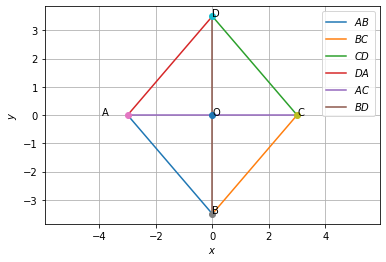
\includegraphics[width=\columnwidth]{solutions/quad/45/figure2.png}
\caption{Rhombus ABCD}
\label{quad/45/fig:Rhombus ABCD}
\end{figure}


\item Construct an isosceles triangle whose base is $a=8$cm and altitude $AD=h=4$cm 
\\
\solution
We obtain the vertices of the rhombus as follows
\begin{align}
\vec{A} = \myvec{-3\\0},
\vec{B} = \myvec{0\\-3.5},
\vec{C} = \myvec{3\\0},
\vec{D} = \myvec{0\\3.5}
\end{align}
which are plotted in Fig. \ref{quad/45/fig:Rhombus ABCD}.
%
\begin{figure}[ht!]
\centering
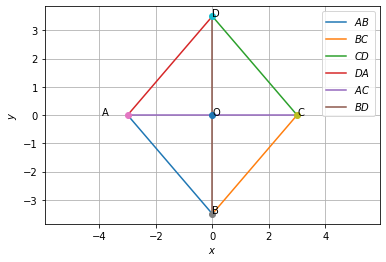
\includegraphics[width=\columnwidth]{solutions/quad/45/figure2.png}
\caption{Rhombus ABCD}
\label{quad/45/fig:Rhombus ABCD}
\end{figure}


\item In $\triangle ABC$,  given that $a+b+c = 11, \angle B = 45^{\degree}$ and $\angle C = 45^{\degree}$, 
find 
$a,b,c$ and sketch the triangle.
\\
\solution
We obtain the vertices of the rhombus as follows
\begin{align}
\vec{A} = \myvec{-3\\0},
\vec{B} = \myvec{0\\-3.5},
\vec{C} = \myvec{3\\0},
\vec{D} = \myvec{0\\3.5}
\end{align}
which are plotted in Fig. \ref{quad/45/fig:Rhombus ABCD}.
%
\begin{figure}[ht!]
\centering
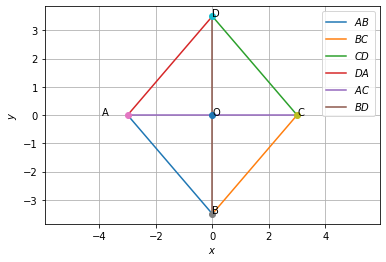
\includegraphics[width=\columnwidth]{solutions/quad/45/figure2.png}
\caption{Rhombus ABCD}
\label{quad/45/fig:Rhombus ABCD}
\end{figure}


\item Draw $\triangle ABC$ with $a = 6, c = 5$ and $\angle B = 60 \degree$. 
\\
\solution
We obtain the vertices of the rhombus as follows
\begin{align}
\vec{A} = \myvec{-3\\0},
\vec{B} = \myvec{0\\-3.5},
\vec{C} = \myvec{3\\0},
\vec{D} = \myvec{0\\3.5}
\end{align}
which are plotted in Fig. \ref{quad/45/fig:Rhombus ABCD}.
%
\begin{figure}[ht!]
\centering
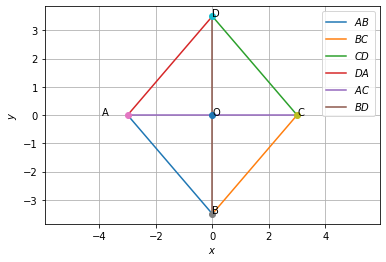
\includegraphics[width=\columnwidth]{solutions/quad/45/figure2.png}
\caption{Rhombus ABCD}
\label{quad/45/fig:Rhombus ABCD}
\end{figure}


\item Draw $\triangle ABC$ with $a = 7, \angle B = 45\degree$ and $\angle A = 105 \degree$. 
\\
\solution
We obtain the vertices of the rhombus as follows
\begin{align}
\vec{A} = \myvec{-3\\0},
\vec{B} = \myvec{0\\-3.5},
\vec{C} = \myvec{3\\0},
\vec{D} = \myvec{0\\3.5}
\end{align}
which are plotted in Fig. \ref{quad/45/fig:Rhombus ABCD}.
%
\begin{figure}[ht!]
\centering
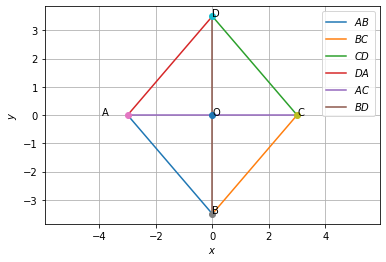
\includegraphics[width=\columnwidth]{solutions/quad/45/figure2.png}
\caption{Rhombus ABCD}
\label{quad/45/fig:Rhombus ABCD}
\end{figure}


\item $\triangle ABC$ is right angled at $\vec{B}$.  If $a = 12$ and $b+c = 18$, find $b,c$ and draw the triangle.
\\
\solution
We obtain the vertices of the rhombus as follows
\begin{align}
\vec{A} = \myvec{-3\\0},
\vec{B} = \myvec{0\\-3.5},
\vec{C} = \myvec{3\\0},
\vec{D} = \myvec{0\\3.5}
\end{align}
which are plotted in Fig. \ref{quad/45/fig:Rhombus ABCD}.
%
\begin{figure}[ht!]
\centering
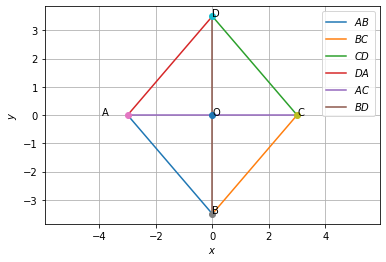
\includegraphics[width=\columnwidth]{solutions/quad/45/figure2.png}
\caption{Rhombus ABCD}
\label{quad/45/fig:Rhombus ABCD}
\end{figure}

%\item Draw $\triangle ABC$ if $AB = 3, AC = 5$ and $\angle C = 30 \degree$.
\item In $\triangle ABC$,  $a = 8, \angle B = 45^{\degree}$ and $c-b = 3.5$.
Sketch $\triangle ABC$.
\\
\solution
We obtain the vertices of the rhombus as follows
\begin{align}
\vec{A} = \myvec{-3\\0},
\vec{B} = \myvec{0\\-3.5},
\vec{C} = \myvec{3\\0},
\vec{D} = \myvec{0\\3.5}
\end{align}
which are plotted in Fig. \ref{quad/45/fig:Rhombus ABCD}.
%
\begin{figure}[ht!]
\centering
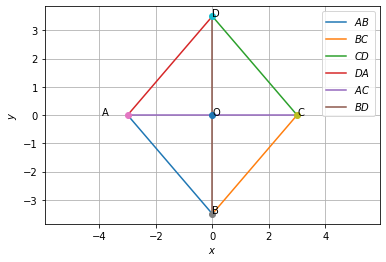
\includegraphics[width=\columnwidth]{solutions/quad/45/figure2.png}
\caption{Rhombus ABCD}
\label{quad/45/fig:Rhombus ABCD}
\end{figure}


\item In $\triangle ABC$,  $a = 6, \angle B = 60^{\degree}$ and $b-c = 2$. 
Sketch $\triangle ABC$.
We obtain the vertices of the rhombus as follows
\begin{align}
\vec{A} = \myvec{-3\\0},
\vec{B} = \myvec{0\\-3.5},
\vec{C} = \myvec{3\\0},
\vec{D} = \myvec{0\\3.5}
\end{align}
which are plotted in Fig. \ref{quad/45/fig:Rhombus ABCD}.
%
\begin{figure}[ht!]
\centering
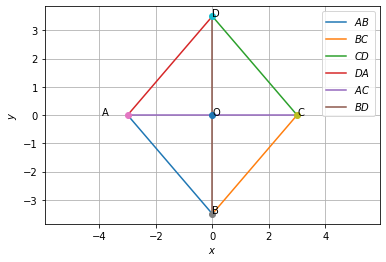
\includegraphics[width=\columnwidth]{solutions/quad/45/figure2.png}
\caption{Rhombus ABCD}
\label{quad/45/fig:Rhombus ABCD}
\end{figure}

\item Draw $\triangle ABC$,  given that $a+b+c = 11, \angle B = 30^{\degree}$ and $\angle C = 90^{\degree}$.
\\
\solution
We obtain the vertices of the rhombus as follows
\begin{align}
\vec{A} = \myvec{-3\\0},
\vec{B} = \myvec{0\\-3.5},
\vec{C} = \myvec{3\\0},
\vec{D} = \myvec{0\\3.5}
\end{align}
which are plotted in Fig. \ref{quad/45/fig:Rhombus ABCD}.
%
\begin{figure}[ht!]
\centering
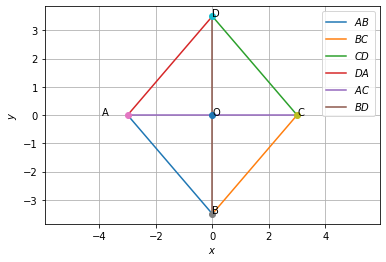
\includegraphics[width=\columnwidth]{solutions/quad/45/figure2.png}
\caption{Rhombus ABCD}
\label{quad/45/fig:Rhombus ABCD}
\end{figure}


\item Construct $\triangle xyz$ where $xy = 4.5, yz = 5$ and $zx = 6$.
\\
\solution
We obtain the vertices of the rhombus as follows
\begin{align}
\vec{A} = \myvec{-3\\0},
\vec{B} = \myvec{0\\-3.5},
\vec{C} = \myvec{3\\0},
\vec{D} = \myvec{0\\3.5}
\end{align}
which are plotted in Fig. \ref{quad/45/fig:Rhombus ABCD}.
%
\begin{figure}[ht!]
\centering
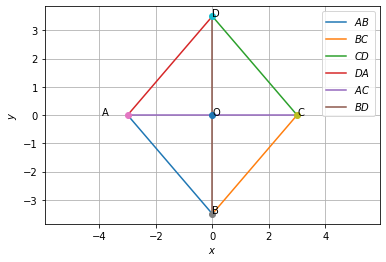
\includegraphics[width=\columnwidth]{solutions/quad/45/figure2.png}
\caption{Rhombus ABCD}
\label{quad/45/fig:Rhombus ABCD}
\end{figure}


\item Draw an equilateral triangle of side $5.5$.
\\
\solution
We obtain the vertices of the rhombus as follows
\begin{align}
\vec{A} = \myvec{-3\\0},
\vec{B} = \myvec{0\\-3.5},
\vec{C} = \myvec{3\\0},
\vec{D} = \myvec{0\\3.5}
\end{align}
which are plotted in Fig. \ref{quad/45/fig:Rhombus ABCD}.
%
\begin{figure}[ht!]
\centering
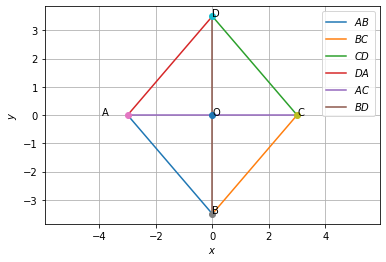
\includegraphics[width=\columnwidth]{solutions/quad/45/figure2.png}
\caption{Rhombus ABCD}
\label{quad/45/fig:Rhombus ABCD}
\end{figure}


\item Draw $\triangle PQR$ with $PQ = 4, QR = 3.5$ and $PR = 4$.  What type of triangle is this?
\\
\solution
We obtain the vertices of the rhombus as follows
\begin{align}
\vec{A} = \myvec{-3\\0},
\vec{B} = \myvec{0\\-3.5},
\vec{C} = \myvec{3\\0},
\vec{D} = \myvec{0\\3.5}
\end{align}
which are plotted in Fig. \ref{quad/45/fig:Rhombus ABCD}.
%
\begin{figure}[ht!]
\centering
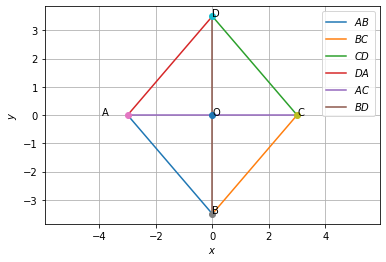
\includegraphics[width=\columnwidth]{solutions/quad/45/figure2.png}
\caption{Rhombus ABCD}
\label{quad/45/fig:Rhombus ABCD}
\end{figure}


\item Construct $\triangle ABC$ such that $AB = 2.5, BC = 6$ and $AC = 6.5$.  Find $\angle B$.
\\
\solution
We obtain the vertices of the rhombus as follows
\begin{align}
\vec{A} = \myvec{-3\\0},
\vec{B} = \myvec{0\\-3.5},
\vec{C} = \myvec{3\\0},
\vec{D} = \myvec{0\\3.5}
\end{align}
which are plotted in Fig. \ref{quad/45/fig:Rhombus ABCD}.
%
\begin{figure}[ht!]
\centering
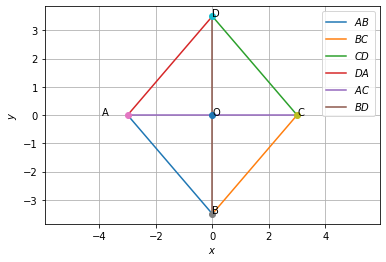
\includegraphics[width=\columnwidth]{solutions/quad/45/figure2.png}
\caption{Rhombus ABCD}
\label{quad/45/fig:Rhombus ABCD}
\end{figure}


\item Construct $\triangle DEF$ such that $DE = 5, DF = 3$ and $\angle D = 90\degree$.
\\
\solution
We obtain the vertices of the rhombus as follows
\begin{align}
\vec{A} = \myvec{-3\\0},
\vec{B} = \myvec{0\\-3.5},
\vec{C} = \myvec{3\\0},
\vec{D} = \myvec{0\\3.5}
\end{align}
which are plotted in Fig. \ref{quad/45/fig:Rhombus ABCD}.
%
\begin{figure}[ht!]
\centering
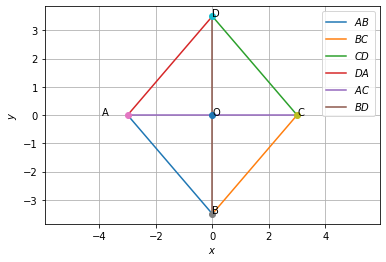
\includegraphics[width=\columnwidth]{solutions/quad/45/figure2.png}
\caption{Rhombus ABCD}
\label{quad/45/fig:Rhombus ABCD}
\end{figure}


\item Construct an isosceles triangle in which the lengths of the equal sides is 6.5 and the angle between them is $110\degree$.
\\
\solution
We obtain the vertices of the rhombus as follows
\begin{align}
\vec{A} = \myvec{-3\\0},
\vec{B} = \myvec{0\\-3.5},
\vec{C} = \myvec{3\\0},
\vec{D} = \myvec{0\\3.5}
\end{align}
which are plotted in Fig. \ref{quad/45/fig:Rhombus ABCD}.
%
\begin{figure}[ht!]
\centering
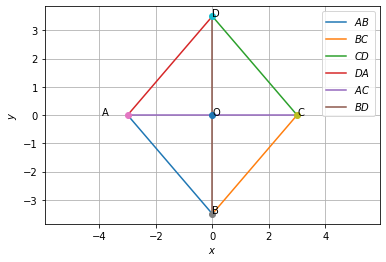
\includegraphics[width=\columnwidth]{solutions/quad/45/figure2.png}
\caption{Rhombus ABCD}
\label{quad/45/fig:Rhombus ABCD}
\end{figure}

\item Construct $\triangle ABC$ given that $\angle A = 60\degree, \angle B = 30\degree$ and $AB = 5.8$.
\\
\solution
From the given information, 
\begin{align}
\angle C = 90^{\degree}
\end{align}
Hence, 
\begin{align}
\vec{A}&=\myvec{0\\c\sin{B}}\\
              &=\myvec{0\\2.9}\\
\vec{B} &=\myvec{c\cos{B}\\0}\\
               &=\myvec {5.02294\\0}\\
\vec{C} &=\myvec{0\\0}
\end{align}
which are used to draw $\triangle ABC$ in Fig. \ref{triangle/20/fig:triangle ABC}.
%
\begin{figure}[!ht]
\centering
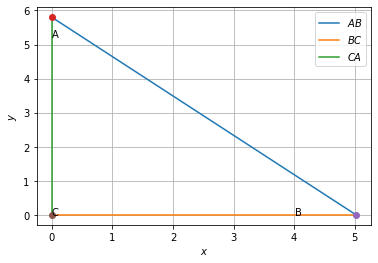
\includegraphics[width=\columnwidth]{solutions/triangle/20/Figure01.png}
\caption{$\triangle ABC$}
\label{triangle/20/fig:triangle ABC}
\end{figure}    

\item Construct  $\triangle LMN$ right angled at $M$ such that $LN = 5$ and $MN = 3$.
 \\
 \solution
We obtain the vertices of the rhombus as follows
\begin{align}
\vec{A} = \myvec{-3\\0},
\vec{B} = \myvec{0\\-3.5},
\vec{C} = \myvec{3\\0},
\vec{D} = \myvec{0\\3.5}
\end{align}
which are plotted in Fig. \ref{quad/45/fig:Rhombus ABCD}.
%
\begin{figure}[ht!]
\centering
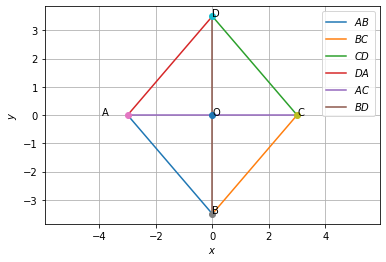
\includegraphics[width=\columnwidth]{solutions/quad/45/figure2.png}
\caption{Rhombus ABCD}
\label{quad/45/fig:Rhombus ABCD}
\end{figure}

\item Construct  $\triangle PQR$ right angled at $Q$ such that $QR = 8$ and $PR = 10$.
\\
\solution

\begin{align}
\because     \vec{A} = b\myvec{\cos C\\ \sin C}, \vec{B} = \myvec{a\\0}, \vec{C} = \myvec{0\\0},
    \end{align}
    substituting the given values, 
    \begin{align}
        \vec{A} = 5\myvec{\cos60\\ \sin60} = \myvec{2.5\\2.5\sqrt3},  \vec{B} = \myvec{7.5\\0},  \vec{C} = \myvec{0\\0}
        \end{align}
    which are plotted in Fig. \ref{constr/july/2Figure}.       

\begin{figure}[!h]
         \centering
         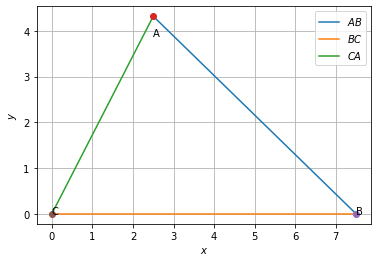
\includegraphics[width= \columnwidth]{solutions/july/2/2/Figures/Figure 1.png}
         \caption{The Constructed triangle}
         \label{constr/july/2Figure}
\end{figure}




\item Construct  right angled $\triangle $ whose hypotenuse  is 6 and one of the legs is 4.
\\
\solution
From the given information,
%
\begin{align}
\angle{C} = \ang{60}
\end{align}
%
Using the sine formula, 
%
\begin{align}
c &= b \brak{\frac{\sin{C}}{\sin{B}}} 
\\
&= 3.3915
\end{align}
%
the vertices of $\triangle ABC$ are
\begin{align}
\vec{A} = \myvec{0 \\ 0},
\vec{B} = c\myvec{\cos{\ang{70}} \\ \sin{\ang{70}}},
\vec{C} = \myvec{3 \\ 0}
\end{align}
and  plotted in Fig. \ref{constr/tri/27/3/fig:triangle ABC}.
%
\begin{figure}[ht]
    \centering
    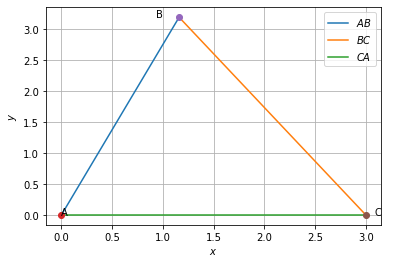
\includegraphics[width=\columnwidth]{solutions/triangle/27/3/Triangle_ABC.PNG}
    \caption{Plot of $\triangle ABC$}
    \label{constr/tri/27/3/fig:triangle ABC}
\end{figure}



\item Construct  an isosceles right angled $\triangle ABC$ right angled at $C$ such $AC = 6$.
\\
\solution

$\because \triangle ABC$ is isosceles, its vertices are
\begin{align}
\vec{C} = \myvec{0\\0},
\vec{A} = \myvec{6\\0}, 
\vec{B} = \myvec{0\\6}
\end{align}
which are used to plot the desired triangle in Fig. \ref{constr/26/fig:right_angle_triangle}.	
%
\begin{figure}[!ht]
\centering
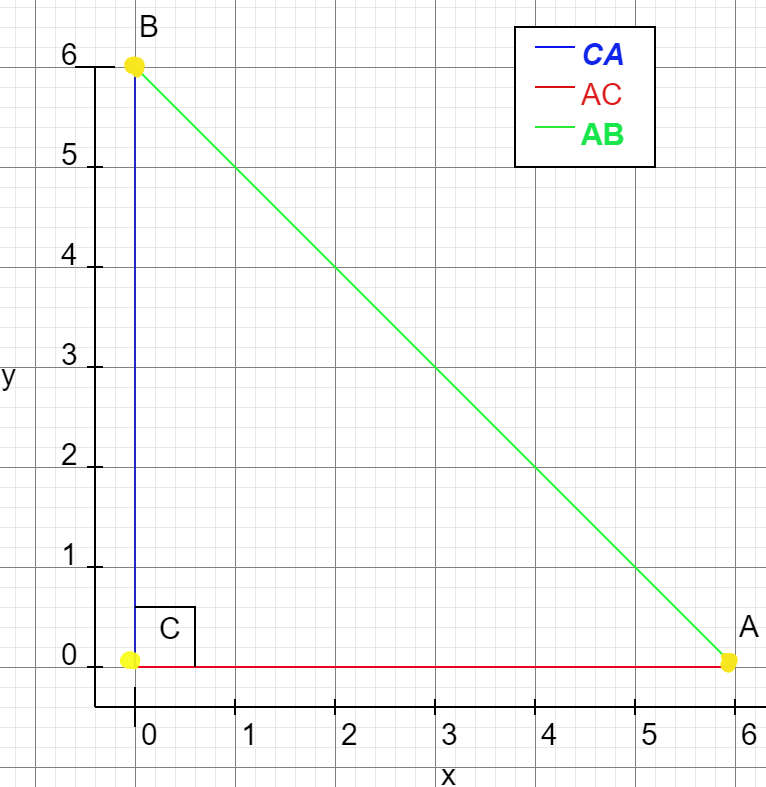
\includegraphics[width=\columnwidth]{solutions/26/diagram-1.png}
\caption{Isosceles Right Angle $\triangle ABC$}
\label{constr/26/fig:right_angle_triangle}	
\end{figure}






%\end{enumerate}


%\section{Quadrilateral}
%\renewcommand{\theequation}{\theenumi}
%\begin{enumerate}[label=\arabic*.,ref=\thesection.\theenumi]
%\numberwithin{equation}{enumi}
	%
%
% \renewcommand{\theequation}{\theenumi}
% \numberwithin{figure}{enumi}

\item Construct parallelogram $ABCD$ 	in Fig. \ref{fig:pgm_sas}	
given that  $BC = 5, AB = 6, \angle C = 85 \degree$.
\begin{figure}[!ht]
	\begin{center}
		\resizebox{\columnwidth}{!}{\input{./figs/quad/pgm_sas.tex}}
	\end{center}
	\caption{Parallelogram Properties}
	\label{fig:pgm_sas}	
\end{figure}
%
\\
\solution $BD$ is found using the cosine formula and $\triangle BDC$ is drawn using the approach in Construction \ref{const:tri_sss} with 
%
\begin{align}
\vec{B} = \myvec{0\\0},
\vec{C} = \myvec{5\\0},
\end{align}
%
Since the diagonals bisect each other, 
%
\begin{align}
\vec{O} &= \frac{\vec{B}+\vec{D}}{2}
\\
\vec{A} &= 2\vec{O} - \vec{C}.
\end{align}
%
$AB$ and $AD$ are then joined to complete the $\parallel$gm.
The python code for  Fig. \ref{fig:pgm_sas} is
\begin{lstlisting}
codes/quad/pgm_sas.py
\end{lstlisting}
%
and 
The equivalent latex-tikz code is
%
\begin{lstlisting}
figs/quad/pgm_sas.tex
\end{lstlisting}
%

\item Draw the $\parallel$gm $ABCD$ in 	Fig. \ref{fig:pgm_sss}	
with $BC = 6, CD = 4.5$ and $BD=7.5$.  Show that it is a rectangle.
\label{const:pgm_sss}
%
\begin{figure}[!ht]
	\begin{center}
		\resizebox{\columnwidth}{!}{\input{./figs/quad/pgm_sss.tex}}
	\end{center}
	\caption{Rectangle}
	\label{fig:pgm_sss}	
\end{figure}
\\
\solution It is easy to verify that 
%Using the approach in Construction\ref{const:tri_sss}, $\triangle BCD$ is drawn with
%
\begin{align}
BD^2=BC^2+C^2
\end{align}
%
Hence, using Baudhayana theorem, 
%
\begin{align}
\angle BCD = 90\degree
\end{align}
%
and  $ABCD$ is a rectangle.
\begin{align}
\vec{A} = \myvec{0\\4.5}
\vec{B} = \myvec{0\\0}
\vec{C} = \myvec{6\\0}
\vec{D} = \myvec{6\\4}
\end{align}
%
The python code for  Fig. \ref{fig:pgm_sss} is
\begin{lstlisting}
codes/quad/pgm_sss.py
\end{lstlisting}
%
and the equivalent latex-tikz code is
%
\begin{lstlisting}
figs/quad/pgm_sss.tex
\end{lstlisting}
%
%
%
%
%
\item Draw the rhombus $BEST$ with $BE = 4.5$ and $ET = 6$. 
\begin{figure}[!ht]
	\begin{center}
		\resizebox{\columnwidth}{!}{\input{./figs/quad/rhom_sss.tex}}
	\end{center}
	\caption{Rhombus}
	\label{fig:rhom_sss}	
\end{figure}
\\
\solution The coordinates of the various points in Fig. \ref{fig:rhom_sss} are obtained as
%
\begin{align}
\vec{O} = \myvec{0\\0},
\vec{B} = \myvec{0\\-4.5}
\\
\vec{E} = \myvec{3\\0},
\vec{S} = \myvec{4.5\\0},
\vec{T} = \myvec{0\\-3}
\end{align}
%
\item A square is a rectangle whose sides are equal.  Draw a square of side 4.5.
\\
\solution The coordinates of the various points in Fig. \ref{fig:square} are obtained as
%
\begin{align}
\vec{A} = \myvec{0\\4.5}
\\
\vec{B} = \myvec{0\\0},
\vec{C} = \myvec{4.5\\0},
\vec{D} = \myvec{4.5\\4.5}
\vec{O} = \frac{\vec{B}+\vec{C}}{2}
%
\end{align}
%
\begin{figure}[!ht]
	\begin{center}
		\resizebox{\columnwidth}{!}{\input{./figs/quad/square.tex}}
	\end{center}
	\caption{Square}
	\label{fig:square}	
\end{figure}

%
%\end{enumerate}

\end{enumerate}

\section{Exercises}
\renewcommand{\thefigure}{\theenumi}
\renewcommand{\theequation}{\theenumi}
\renewcommand{\thetable}{\theenumi}
\begin{enumerate}[label=\thesection.\arabic*.,ref=\thesection.\theenumi]
\numberwithin{equation}{enumi}
\numberwithin{figure}{enumi}
\numberwithin{table}{enumi}
%\renewcommand{\theequation}{\theenumi}
%\begin{enumerate}[label=\thesubsection.\arabic*.,ref=\thesubsection.\theenumi]
%%\begin{enumerate}[label=\arabic*.,ref=\thesection.\theenumi]
%\renewcommand{\thefigure}{\theenumi}    
%\numberwithin{equation}{enumi}
% \numberwithin{equation}{enumi}
% \numberwithin{figure}{enumi}
% \numberwithin{table}{enumi}



\item Construct $\triangle PQR$, given that $PQ = 3, QR = 5.5$ and $\angle PQR = 60 \degree$.
\\
\solution
\begin{align}
    \because \vec{P} = r\myvec{\cos Q\\ \sin Q}, \vec{Q} = \myvec{0\\0}, \vec{R} = \myvec{p\\0}
    \end{align}
    from the given information, 
    \begin{align}
    \vec{P} = 3\myvec{\cos60\\ \sin60} = \frac{3}{2}\myvec{1\\\sqrt3},  \vec{Q} = \myvec{0\\0},  \vec{R} = \myvec{5.5\\0}
    \end{align}
and plotted in Fig.              \ref{constr/july/1Figure}.
    
    
\begin{figure}[!ht]
\centering
         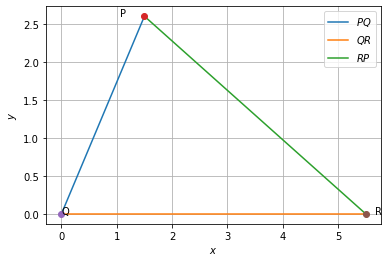
\includegraphics[width= \columnwidth]{solutions/july/2/1/figure1.png}
         \caption{The Constructed triangle}
         \label{constr/july/1Figure}
\end{figure}






%
\item Construct $\triangle ABC$  with $BC = 7.5, AC = 5$ and $\angle C = 60\degree$.
\\
\solution

\begin{align}
\because     \vec{A} = b\myvec{\cos C\\ \sin C}, \vec{B} = \myvec{a\\0}, \vec{C} = \myvec{0\\0},
    \end{align}
    substituting the given values, 
    \begin{align}
        \vec{A} = 5\myvec{\cos60\\ \sin60} = \myvec{2.5\\2.5\sqrt3},  \vec{B} = \myvec{7.5\\0},  \vec{C} = \myvec{0\\0}
        \end{align}
    which are plotted in Fig. \ref{constr/july/2Figure}.       

\begin{figure}[!h]
         \centering
         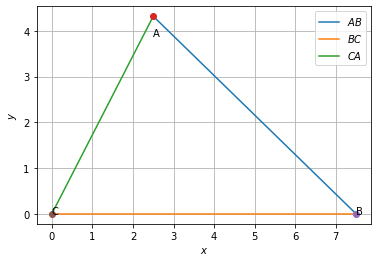
\includegraphics[width= \columnwidth]{solutions/july/2/2/Figures/Figure 1.png}
         \caption{The Constructed triangle}
         \label{constr/july/2Figure}
\end{figure}




\item Construct $\triangle XYZ$ if $XY = 6, \angle X = 30\degree$ and $\angle Y = 100 \degree$.
\item If $AC = 7, \angle A = 60\degree$ and $\angle B = 50 \degree$, can you draw the triangle?
%
\solution
From the given information, 
To find angle C:
\begin{align}
\angle{C} = \ang{70}
\end{align}
and 
\begin{align}
  a&= b\brak{\frac{\sin{A}}{\sin{B}}} 
\\
  &= 7.913611
  \end{align}
%  
Thus, the coordinates are 
\begin{align}
  \vec{C} =\myvec{0 \\ 0},
  \vec{B} =a\myvec{\cos{\ang{70}} \\ \sin{\ang{70}}},
  \vec{A} =\myvec{7 \\ 0}
  \end{align}
  
\begin{figure}[!h]
\centering
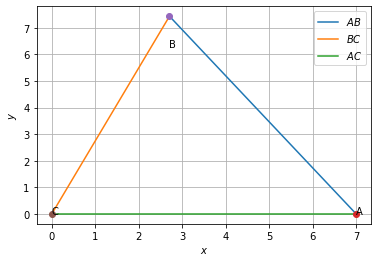
\includegraphics[width=\columnwidth]{solutions/july/2/4/Figure 1.jpeg}
\caption{$\triangle ABC$}
\label{fig:triangle}	
\end{figure}
To find side $a$
The vertices of $\triangle ABC$ are
Lines AB,BC,CA are then generated and plotted using these coordinates to construct $\triangle ABC$
Plot of the $\triangle ABC$:

\end{document}


\item Construct $\triangle PQR$ if $PQ = 5, \angle Q = 105 \degree$ and $\angle R = 40 \degree$.
\item Can you construct $\triangle DEF$ such that $EF = 7.2, \angle E = 110\degree$ and $\angle F = 180\degree$?
\item Construct the  triangles in Table \ref{table:triangle_const_exercises}.
\begin{table}[!ht]
\centering
\input{./chapters/constr/Triangle}
\caption{}
\label{table:triangle_const_exercises}
\end{table}
\solution
\begin{enumerate}
    \item
    \item 
    \solution
    We obtain the vertices of the rhombus as follows
\begin{align}
\vec{A} = \myvec{-3\\0},
\vec{B} = \myvec{0\\-3.5},
\vec{C} = \myvec{3\\0},
\vec{D} = \myvec{0\\3.5}
\end{align}
which are plotted in Fig. \ref{quad/45/fig:Rhombus ABCD}.
%
\begin{figure}[ht!]
\centering
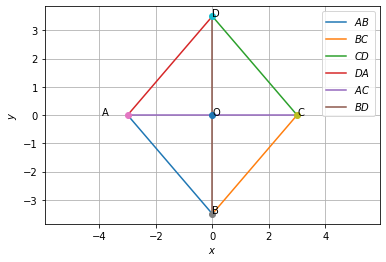
\includegraphics[width=\columnwidth]{solutions/quad/45/figure2.png}
\caption{Rhombus ABCD}
\label{quad/45/fig:Rhombus ABCD}
\end{figure}

    \item 
    \solution
    From the given information,
%
\begin{align}
\angle{C} = \ang{60}
\end{align}
%
Using the sine formula, 
%
\begin{align}
c &= b \brak{\frac{\sin{C}}{\sin{B}}} 
\\
&= 3.3915
\end{align}
%
the vertices of $\triangle ABC$ are
\begin{align}
\vec{A} = \myvec{0 \\ 0},
\vec{B} = c\myvec{\cos{\ang{70}} \\ \sin{\ang{70}}},
\vec{C} = \myvec{3 \\ 0}
\end{align}
and  plotted in Fig. \ref{constr/tri/27/3/fig:triangle ABC}.
%
\begin{figure}[ht]
    \centering
    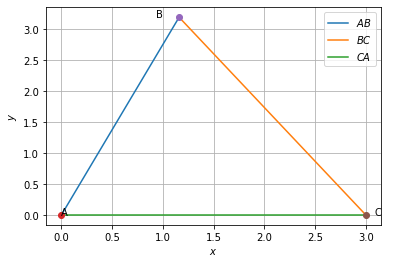
\includegraphics[width=\columnwidth]{solutions/triangle/27/3/Triangle_ABC.PNG}
    \caption{Plot of $\triangle ABC$}
    \label{constr/tri/27/3/fig:triangle ABC}
\end{figure}


        
\end{enumerate}
%

 %\renewcommand{\theequation}{\theenumi}
%\begin{enumerate}[label=\thesubsection.\arabic*.,ref=\thesubsection.\theenumi]
%%\begin{enumerate}[label=\arabic*.,ref=\thesection.\theenumi]
%\numberwithin{equation}{enumi}


\item Construct a quadrilateral $ABCD$ such that $AB=5, \angle A = 50\degree, AC = 4, BD = 5$ and $AD = 6$.
\\
\solution 
\begin{enumerate}
    \item Given point $\vec{P} = \myvec{-4\\3}$ and slope $m = \frac{1}{2}$.
    The direction vector is $\vec{m} = \myvec{2\\1}$.  
    Hence, the normal vector
    \begin{align}
    \label{linform/2/14/eq:line_norm_dir}
    \vec{n} &= \myvec{0&-1\\1&0}\vec{m} 
    \\
    &= \myvec{-1\\2}
    \end{align}
    The equation of the line in terms of the normal vector is then obtained as
    \begin{align}
    \label{linform/2/14/eq:line_norm_vec}
    \vec{n}^T\brak{\vec{x}-\vec{A}} &= 0
    \\
    \implies \myvec{-1 & 2} \vec{x} &= 10
    \end{align}
    See Fig.     \ref{linform/2/14/Plot of Line $AB$ (Part-1)}
    \begin{figure}[ht]
    \centering
    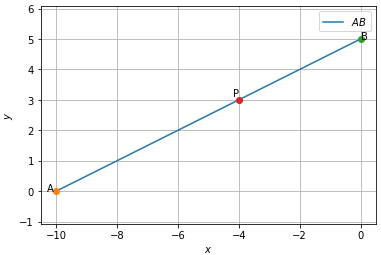
\includegraphics[width=\columnwidth]{solutions/su2021/2/14/Line_Plot_Part1.PNG}
    \caption{Plot of Line $AB$ (Part-1)}
    \label{linform/2/14/Plot of Line $AB$ (Part-1)}
    \end{figure}
    \item Given point $\vec{P} = \myvec{2\\2\sqrt{3}}$.From the given information we have, $\tan75\degree =m = \frac{\sqrt{3}+1}{\sqrt{3}-1}$.
    The direction vector is $\vec{m} = \myvec{1\\\tan75\degree}$.  
    Hence, the normal vector
    \begin{align}
    \label{linform/2/14/eq:line_norm_dir2}
    \vec{n} &= \myvec{0&-1\\1&0}\vec{m} 
    \\
    &= \myvec{-\tan75\degree\\1}
    \end{align}
    The equation of the line in terms of the normal vector is then obtained as
    \begin{align}
    \label{linform/2/14/eq:line_norm_vec2}
    \vec{n}^T\brak{\vec{x}-\vec{A}} &= 0
    \\
    \implies \myvec{-\sqrt{3}+1 &\sqrt{3}-1}  \vec{x} &= -4\brak{\sqrt{3}-1}
    \end{align}
    See Fig. \ref{linform/2/14/Plot of Line $AB$ (Part-2)}

    \begin{figure}[ht]
    \centering
    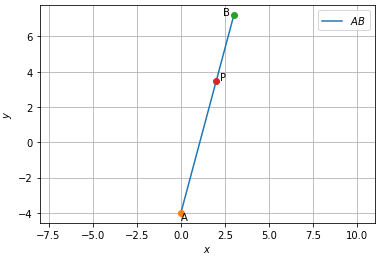
\includegraphics[width=\columnwidth]{solutions/su2021/2/14/Line_Plot_Part2.PNG}
    \caption{Plot of Line $AB$ (Part-2)}
    \label{linform/2/14/Plot of Line $AB$ (Part-2)}
    \end{figure}
\end{enumerate}
\item Construct $PQRS$ where $PQ = 4, QR = 6, RS = 5, PS = 5.5$ and $PR = 7$.
\item Draw $JUMP$ with $JU = 3.5, UM=4, MP = 5, PJ =4.5$ and $PU = 6.5$
\item Construct a quadrilateral $ABCD$ such that $BC=4.5,  AC = 5.5, CD = 5, BD = 7$ and $AD = 5.5$.
\item Can you construct a quadrilateral $PQRS$ with $PQ=3, RS=3, PS=7.5, PR=8$ and $SQ=4$?
\\
\solution 
  
  If we expand the probabilities given further more by substituting the value of x and only considering 0 to 4 hours as the probability of studying in the remaining hours is zero, we get
  
  \begin{table}[ht]
  
 \centering
  
  \begin{tabular}{|c|c|c|c|c|c|}
    \hline
    x &  0 & 1 & 2 & 3 & 4\\
    \hline
    $\Pr\brak{X=x}$ & 0.1& k& 2k & 2k & k\\
    \hline
    
\end{tabular}
\caption{Given probabilities}
\label{Table_1}
\end{table}
we also know that,
\begin{align}
    \sum_{k = 0}^4 \Pr\brak{X = k} = 1 \label{eq 2.0.1}
\end{align}

By substituting the probabilities in \eqref{eq 2.0.1}
\begin{align}
& \implies 0.1 + k + 2k + 2k + k = 1 \\
& \implies 6k = 0.9 \label{eq 2.0.3}
\end{align}

Therefore, from \eqref{eq 2.0.3}
\begin{align}
    k = 0.15
\end{align}
  
 So from \ref{Table_1}
  \begin{table}[ht]
  
  \centering
  \begin{tabular}{|c|c|c|c|c|c|}
    \hline
    x &  0 & 1 & 2 & 3 & 4\\
    \hline
    $\Pr\brak{X=x}$ & 0.1& 0.15& 0.3 & 0.3 & 0.15\\
    \hline
    
\end{tabular} 
\caption{Probabilities after finding k}
\end{table}

\begin{figure}[ht]
    \centering
    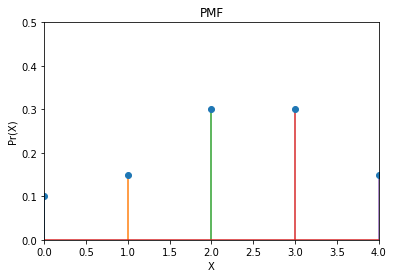
\includegraphics[width=\columnwidth]{solutions/5/28/Figures/PMF.png}
    \caption{Probability Mass Function (PMF)}
    \label{Figure_1}
\end{figure}

We know that, Cumulative Distributive Function (CDF) 
\begin{align}
    F(x) = \Pr\brak{X \le x}
\end{align}

\begin{table}[ht]
  
  \centering
  \begin{tabular}{|c|c|c|c|c|c|}
    \hline
    x &  0 & 1 & 2 & 3 & 4\\
    \hline
    $F(X)$ & 0.1& 0.25& 0.55 & 0.85 & 1\\
    \hline
    
\end{tabular} 
\caption{CDF}
\label{Table_2}
\end{table}

\begin{figure}[ht]
    \centering
    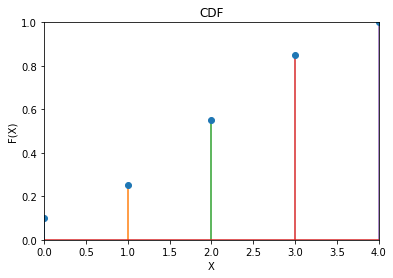
\includegraphics[width=\columnwidth]{solutions/5/28/Figures/CDF.png}
    \caption{Cumulative Distributive Function (CDF)}
    \label{Figure_2}
\end{figure}

And also, 
\begin{align}
     \Pr\brak{x < X \le y} = F\brak{y} - F\brak{x} \label{eq 2.0.6}
\end{align}
         \begin{enumerate}
        \item Probability of studying at least two hours 
           \begin{align}
            & \implies \sum_{k = 2}^4 \Pr\brak{X = k} = \Pr\brak{X \ge 2}\\
            & \implies \Pr\brak{1 < X \le 4} 
        \end{align}
        From \eqref{eq 2.0.6} and \eqref{Table_2}
        \begin{align}
            & = F(4) - F(1)\\
            & = 1 - 0.25\\
            & = 0.75
        \end{align}
        
        \item Probability of studying exactly two hours
        \begin{align}
            & = \Pr\brak{X = 2}\\
            & = 0.3
        \end{align}
        
        \item Probability of studying at most two hours 
        \begin{align}
          & \implies \sum_{k = 0}^2  \Pr\brak{X = k} = \Pr \brak{X \le 2}
         \end{align}
        From \eqref{Table_2}
        \begin{align}
            & = F(2)\\
            & = 0.55
        \end{align}
    \end{enumerate}
  
    \begin{table}[ht]
   
    \centering
  \begin{tabular}{|c|c|c|}
    \hline
    $\Pr\brak{X \geq 2}$ &  $\Pr \brak{X = 2}$ & $\Pr\brak{X \leq 2}$\\
    \hline
     0.75& 0.3& 0.55 \\
    \hline
    Case 1 &Case 2 &Case 3\\
    \hline
\end{tabular} 
 \caption{Final solution}
 \label{Table_3}
\end{table}

\begin{figure}[ht]
    \centering
    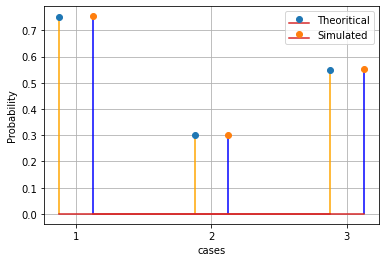
\includegraphics[width=\columnwidth]{solutions/5/28/Figures/stem.png}
    \caption{Simulation and Theoretical Comparison}
    \label{Figure_3}
\end{figure}


\item Construct $LIFT$ such that $LI = 4, IF = 3, TL = 2.5, LF = 4.5, IT=4$.
\item Draw $GOLD$ such that $OL=7.5, GL=6, GD=6, LD = 5, OD = 10$.
\\
\solution 
We obtain the vertices of the rhombus as follows
\begin{align}
\vec{A} = \myvec{-3\\0},
\vec{B} = \myvec{0\\-3.5},
\vec{C} = \myvec{3\\0},
\vec{D} = \myvec{0\\3.5}
\end{align}
which are plotted in Fig. \ref{quad/45/fig:Rhombus ABCD}.
%
\begin{figure}[ht!]
\centering
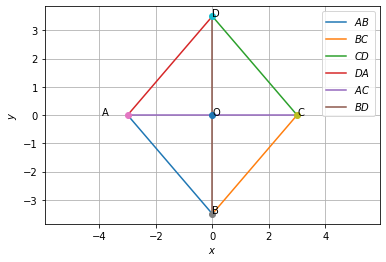
\includegraphics[width=\columnwidth]{solutions/quad/45/figure2.png}
\caption{Rhombus ABCD}
\label{quad/45/fig:Rhombus ABCD}
\end{figure}


\item DRAW rhombus $BEND$ such that $BN = 5.6$, $DE = 6.5$.
\item construct a quadrilateral MIST where $MI = 3.5, IS = 6.5, \angle M = 75 \degree, \angle I = 105 \degree$ and $\angle S = 120 \degree$.
\item Can you construct the above quadrilateral MIST if $\angle M = 100 \degree$ instead of $75 \degree$.
\item Can you constrcut the quadrilateral PLAN if $PL = 6, LA = 9.5, \angle P = 75 \degree, \angle L = 150 \degree$ and $\angle A = 140 \degree$?
\item Construct $MORE$ where $MO = 6, OR = 4.5, \angle M = 60 \degree, \angle O = 105 \degree, \angle R = 105 \degree$.
\item Construct $PLAN$ where $PL = 4, LA = 6.5, \angle P = 90 \degree, \angle A = 110\degree$ and $\angle N = 85\degree$.
\item Draw  rectangle $OKAY$ with $OK = 7$ and $KA = 5$.
\item Construct $ABCD $, where $AB = 4, BC = 5, Cd = 6.5, \angle B = 105 \degree$ and $\angle C = 80\degree$.
\\
\solution 

Let 
    \begin{align}
    &\angle B= 105\degree=\theta \label{quad/42/eq1}
    \\
    &\angle C= 80\degree=\alpha \label{quad/42/eq2}
    \\
    &\norm{\vec{A}-\vec{B}} =4=p \label{quad/42/eq3}
    \\
    &\norm{\vec{C}-\vec{B}} =5=q \label{quad/42/eq4}
    \\
     &\norm{\vec{D}-\vec{C}} =6.5=r \label{quad/42/eq5}
    \end{align}
and 
\begin{align}
    &\vec{B}=\myvec{0\\0}, \vec{C}=\myvec{5\\0}
\end{align}

\begin{lemma}
\label{quad/42/lemma}
\begin{align}
  & \vec{A} = p \vec{b}  \quad \brak{\because \vec{B}=\myvec{0\\0}} \label{quad/42/eq a}
\\
  & \vec{D} =\vec{C} + r \vec{c} \label{quad/42/eq b}
\end{align}
where 
\begin{align}
 \vec{b} = \myvec{\cos B \\ \sin B } ,\vec{c} = \myvec{\cos C\\ \sin C }
\end{align}
\end{lemma}
Thus, 
\begin{align}
 \vec{A} &=4\myvec{\cos 105 \\\sin 105 }
\\
&=\myvec{-1.03\\3.86}
\end{align}
and 
\begin{align}
\vec{D} &=\myvec{5\\0} + 6.5\myvec{\cos 80 \\\sin 80 }
\\
&=\myvec{6.12\\6.39}
\end{align}
which are then used to plot Fig. \ref{quad/42/fig:Quadrilateral ABCD}	
\begin{figure}[!ht]
\centering
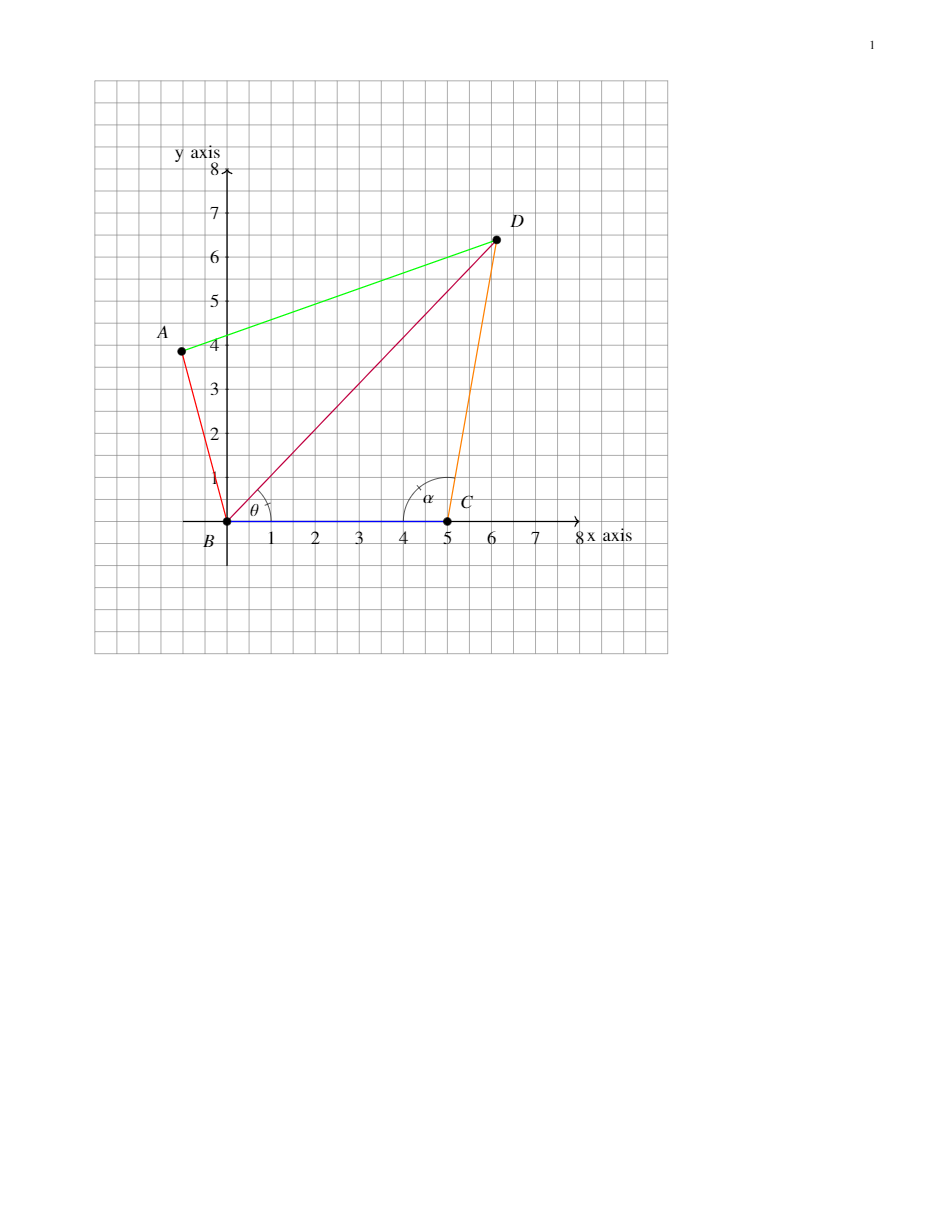
\includegraphics[ width=\columnwidth]{solutions/quad/42/FIGURE.png}
\caption{Quadrilateral ABCD}
\label{quad/42/fig:Quadrilateral ABCD}	
\end{figure}

%
\item Construct $DEAR$ with $DE = 4, EA = 5, AR = 4.5, \angle E = 60 \degree$ and $\angle A = 90 \degree$.
\\
\solution 
We obtain the vertices of the rhombus as follows
\begin{align}
\vec{A} = \myvec{-3\\0},
\vec{B} = \myvec{0\\-3.5},
\vec{C} = \myvec{3\\0},
\vec{D} = \myvec{0\\3.5}
\end{align}
which are plotted in Fig. \ref{quad/45/fig:Rhombus ABCD}.
%
\begin{figure}[ht!]
\centering
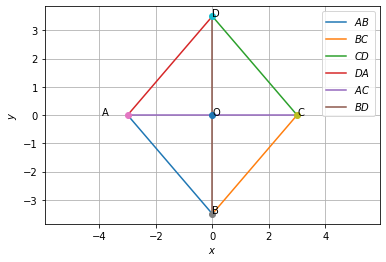
\includegraphics[width=\columnwidth]{solutions/quad/45/figure2.png}
\caption{Rhombus ABCD}
\label{quad/45/fig:Rhombus ABCD}
\end{figure}


\item Construct $TRUE$ with $TR = 3.5, RU = 3, UE = 4 \angle R = 75\degree$ and $\angle U = 120\degree$.
\\
\solution 
We obtain the vertices of the rhombus as follows
\begin{align}
\vec{A} = \myvec{-3\\0},
\vec{B} = \myvec{0\\-3.5},
\vec{C} = \myvec{3\\0},
\vec{D} = \myvec{0\\3.5}
\end{align}
which are plotted in Fig. \ref{quad/45/fig:Rhombus ABCD}.
%
\begin{figure}[ht!]
\centering
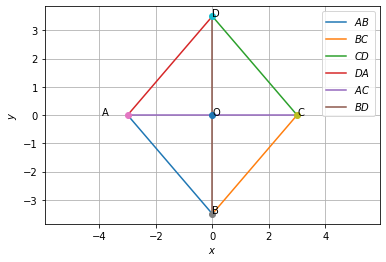
\includegraphics[width=\columnwidth]{solutions/quad/45/figure2.png}
\caption{Rhombus ABCD}
\label{quad/45/fig:Rhombus ABCD}
\end{figure}




\item Can you construct a rhombus $ABCD$ with $AC = 6$ and $BD = 7$?
\\
\solution 
We obtain the vertices of the rhombus as follows
\begin{align}
\vec{A} = \myvec{-3\\0},
\vec{B} = \myvec{0\\-3.5},
\vec{C} = \myvec{3\\0},
\vec{D} = \myvec{0\\3.5}
\end{align}
which are plotted in Fig. \ref{quad/45/fig:Rhombus ABCD}.
%
\begin{figure}[ht!]
\centering
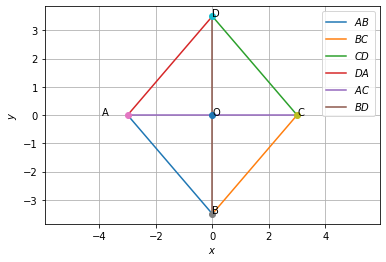
\includegraphics[width=\columnwidth]{solutions/quad/45/figure2.png}
\caption{Rhombus ABCD}
\label{quad/45/fig:Rhombus ABCD}
\end{figure}


\item Draw a square $READ$ with $RE = 5.1$.
\\
\solution 
The centers and radii of the two circles without any loss of generality are given in Table \ref{constr/55/tab:table1}
%
\begin{table}[!ht]
\begin{center}
\begin{tabular}{ | m{2cm} | m{2cm} | m{2cm} |} 
\hline
 & Circle 1 & Circle 2 \\
\hline
Centre  & $\vec{A}$=\myvec{0\\0} & $\vec{B}$=\myvec{3\\0} \\ 
\hline
Radius & $r_{1}=r_{2}=3$  \\ 
\hline
\end{tabular}
\end{center}
\caption{Input values}
\label{constr/55/tab:table1}

\end{table}

% The choice for $\vec{A}$ and $\vec{B}$ is valid as:
% \begin{align}
% \norm{\vec{B}-\vec{A}} = \norm{\vec{A}-\vec{B}}=\norm{\vec{B}}  = 3 \quad \brak{\because \vec{A}=0}
% \end{align}

Let 
\begin{align}
\vec{u}=\myvec{\cos \theta\\  \sin \theta},  \theta \in \sbrak{0,2\pi}.
\end{align}

Then on Circle 1  and Circle 2 are  given by 
\begin{align}
\vec{x}&=\vec{A}+r\vec{u}
\\
\vec{x}&=\vec{B}+r\vec{u}
\end{align}

Fig. \ref{constr/55/fig:circle} is plotted using the above equations.
%
\begin{figure}[!ht]
\centering
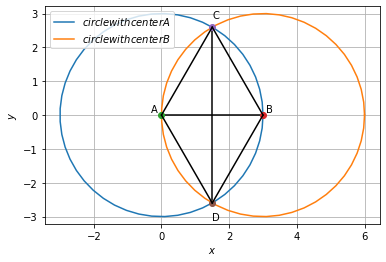
\includegraphics[width=\columnwidth]{solutions/55/Figures/figure3.png}
\caption{Circles with their points of intersection}
\label{constr/55/fig:circle}	
\end{figure}
Fig. \ref{constr/55/fig:circle} 

The general equation of Circle 1 is given by 
\begin{align}
    \norm{\vec{x}-\vec{A}}^2 &= r^2
    \\
\vec{x}^{\top}\vec{x} - 2\vec{A}^{\top}\vec{x} + \norm{\vec{A}}^2 -r_{1}^2 &= 0\label{constr/55/eq:14}
\end{align}
Similarly, for Circle 2,
\begin{align}
\vec{x}^{\top}\vec{x} - 2\vec{B}^{\top}\vec{x} + \norm{\vec{B}}^2 -r_{2}^2 = 0\label{constr/55/eq:15}
\end{align}
Subtracting \eqref{constr/55/eq:15} from \eqref{constr/55/eq:14},
\begin{align}
2\vec{B}^{\top}\vec{x}=\norm{\vec{B}}^2
\\
\myvec{1&0}\vec{x}=\frac{3}{2}
\end{align}
which can be expressed as
\begin{align}
\vec{x} &=\frac{1}{2}\myvec{3\\ 0} + \lambda \myvec{0\\1}\label{constr/55/eq:19}\\
&=\vec{q}+\lambda\vec{m} \text{ where}\label{constr/55/eq:20}\\
\vec{q}&=\myvec{1.5\\ 0},
\vec{m}=\myvec{0\\1}
\end{align}
Substituting \eqref{constr/55/eq:20} in \eqref{constr/55/eq:14}
\begin{align}
\norm{\vec{x}}^2=r^2\quad \brak{\because \vec{A}=0}
\\
\norm{\vec{q}+\lambda\vec{m}}^2=r^2\\
(\vec{q}+\lambda \vec{m})^{\top}(\vec{q}+\lambda \vec{m})=r^2\\
\implies \vec{q}^{\top}(\vec{q}+\lambda \vec{m})+\lambda \vec{m}^{\top}(\vec{q}+\lambda \vec{m})=r^2
\\
\implies \norm{\vec{q}}^2+\lambda\vec{q}^{\top}\vec{m}+\lambda\vec{m}^{\top}\vec{q}+\lambda^2\norm{\vec{m}}^2=r^2
\\
\implies \norm{\vec{q}}^2+2\lambda\vec{q}^{\top}\vec{m}+\lambda^2\norm{\vec{m}}^2=r^2 
% \\
% \implies \lambda(\lambda\norm{\vec{m}}^2+2\vec{q}^{\top}\vec{m})=r^2-\norm{\vec{q}}^2\\
% \implies\lambda^2\norm{\vec{m}}^2=9-\norm{\vec{q}}^2
\\
\implies \lambda=\pm \sqrt{\frac{9-\norm{\vec{q}}^2}{\norm{\vec{m}}^2}} \quad \because \vec{q}^{\top}\vec{m} = 0
% \lambda^2=6.75\\
% \lambda=+\sqrt{6.75},-\sqrt{6.75}
\end{align}
Substituting the value of $\lambda$ in \eqref{constr/55/eq:20},
\begin{align}
%\vec{x}=\vec{q}+\lambda\vec{m}\\
\vec{C}&=\vec{q}+\lambda\vec{m}\\
\vec{D}&=\vec{q}-\lambda\vec{m} \\
\implies (\vec{A}-\vec{B})^{\top}(\vec{C}-\vec{D})
&=2\myvec{-3&0}\myvec{0\\\sqrt{6.75}}
\\
&=0
\\
\implies AB\perp CD
\end{align}


% We have $\vec{C}$ and $\vec{D}$ as points of intersection and $r_{1}=r_{2}$.So,
% \begin{align}
% \norm{\vec{C}-\vec{A}}^2 = \norm{\vec{C}-\vec{B}}^2
% \end{align}
% \begin{align}
% \implies(\vec{C}-\vec{A})^{\top}(\vec{C}-\vec{A})=(\vec{C}-\vec{B})^{\top}(\vec{C}-\vec{B})
% \\
% \implies \vec{A}^{\top}\vec{C}-\vec{B}^{\top}\vec{C}=\vec{C}^{\top}\vec{B}-\vec{C}^{\top}\vec{A}+\norm{\vec{A}}^2-\norm{\vec{B}}^2 
% \end{align}
% \begin{align}
% \implies2\times \vec{A}^{\top}\vec{C}-2\times\vec{B}^{\top}\vec{C}=\norm{\vec{A}}^2-\norm{\vec{B}}^2 \label{constr/55/eq:1}
% \end{align}
% Similarly,using:
% \begin{align}
% \norm{\vec{D}-\vec{A}}^2 = \norm{\vec{D}-\vec{B}}^2
% \end{align}
% We get:
% \begin{align}
% 2\times \vec{A}^{\top}\vec{D}-2\times\vec{B}^{\top}\vec{D}=\norm{\vec{A}}^2-\norm{\vec{B}}^2 \label{constr/55/eq:2}
% \end{align}

% Subtracting equation \ref{constr/55/eq:2} from equation \ref{constr/55/eq:1}:
% \begin{align}
% 2\times(\vec{A}^{\top}-\vec{B}^{\top})(\vec{C}-\vec{D})=0
% \\
% \implies (\vec{A}-\vec{B})^{\top}(\vec{C}-\vec{D})=0
% \\
% \implies AB\perp CD
% \end{align}

\item Draw a rhombus who diagonals are $5.2$ and $6.4$.
\\
\solution 
We obtain the vertices of the rhombus as follows
\begin{align}
\vec{A} = \myvec{-3\\0},
\vec{B} = \myvec{0\\-3.5},
\vec{C} = \myvec{3\\0},
\vec{D} = \myvec{0\\3.5}
\end{align}
which are plotted in Fig. \ref{quad/45/fig:Rhombus ABCD}.
%
\begin{figure}[ht!]
\centering
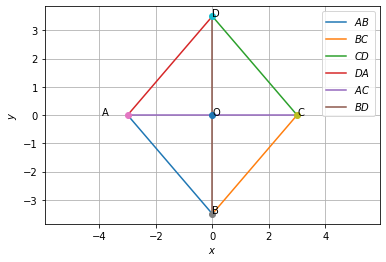
\includegraphics[width=\columnwidth]{solutions/quad/45/figure2.png}
\caption{Rhombus ABCD}
\label{quad/45/fig:Rhombus ABCD}
\end{figure}


\item Draw a rectangle with adjacent sides $5$ and $4$.
\\
\solution 
We obtain the vertices of the rhombus as follows
\begin{align}
\vec{A} = \myvec{-3\\0},
\vec{B} = \myvec{0\\-3.5},
\vec{C} = \myvec{3\\0},
\vec{D} = \myvec{0\\3.5}
\end{align}
which are plotted in Fig. \ref{quad/45/fig:Rhombus ABCD}.
%
\begin{figure}[ht!]
\centering
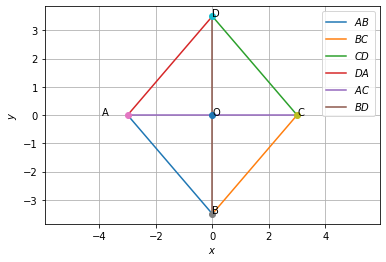
\includegraphics[width=\columnwidth]{solutions/quad/45/figure2.png}
\caption{Rhombus ABCD}
\label{quad/45/fig:Rhombus ABCD}
\end{figure}


\item Draw a parallelogram $OKAY$ with $OK = 5.5$ and $KA = 4.2$.
\\
\solution  There are infinite number of parallelograms that can be draw.  For a unique parallelogram, one angle
needs to be specified.

\item Construct a kite $EASY$ if $AY = 8, EY = 4$ and $SY = 6$.


%\end{enumerate}
%

 %\renewcommand{\theequation}{\theenumi}
%\begin{enumerate}[label=\thesubsection.\arabic*.,ref=\thesubsection.\theenumi]
%%\begin{enumerate}[label=\arabic*.,ref=\thesection.\theenumi]
%\numberwithin{equation}{enumi}

\item Draw a circle of diameter 6.1

\item With the same centre $\vec{O}$,  draw two circles of radii 4 and 2.5
\\
\solution


All input values required to plot Fig. \ref{constr/52/tab:table1} are given in Table \ref{constr/52/tab:table1} as shown below

\begin{table}[!ht]
\begin{center}
    \resizebox{\columnwidth}{!}{
\begin{tabular}{ | m{2cm} | m{1.5cm}| m{2cm} | m{1.5cm} |} 
\hline
& Symbols & Circle1 & Circle2 \\
\hline
Centre & $\vec{O}$ & \myvec{0\\0} & \myvec{0\\0} \\ 
\hline
Radius & $r_{1}$,$r_{2}$ & 2.5 & 4 \\ 
\hline
Polar coordinate & $\vec{C}_{1}$,$\vec{C}_{2}$ & 2.5\myvec{\cos \theta\\  \sin \theta} & 4\myvec{\cos \theta\\  \sin \theta} \\
\hline
Angle & $\theta$ & 0-2$\pi$ & 0-2$\pi$ \\
\hline
\end{tabular}
    }
\end{center}
\caption{Input values}
\label{constr/52/tab:table1}
\end{table}


\begin{figure}[!ht]
\centering
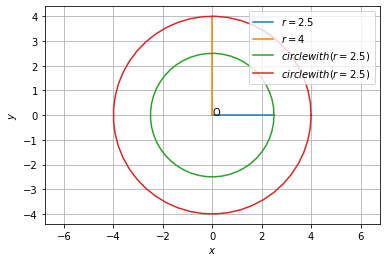
\includegraphics[width=\columnwidth]{solutions/52/Figure3.png}
\caption{Concentric circles with centre as origin and radii 2.5 and 4 respectively}
\label{constr/52/fig:circle}	
\end{figure}


}
\item Draw a circle with centre $\vec{B}$ and radius 6.  If $\vec{C}$ be  a point 10 units  away from its 
centre, construct the pair of tangents $AC$ and $CD$ to the 
circle.
\item Draw a circle of radius 3 and any two of its diameters.  Draw the ends of these diameters. What figure do you get?
\item Let $\vec{A}$ and $\vec{B}$ be the centres of two circles of equal radii 3 such that each one of them passes through the centre of the other.  Let them intersect at $\vec{C}$ and $\vec{D}$.  Is $AB \perp CD$?

\item Construct a tangent to a circle of radius 4 units from a point on the concentric circle of radius 6 
units.
\\
\solution Take the centre of both circles to be at the origin.  
\item Draw a circle of radius 3 units. Take  two points $\vec{P}$ and $\vec{Q}$ on one of its extended 
diameter each at a distance of 7 units from its centre. Draw tangents to the circle from these two points 
$\vec{P}$ and $\vec{Q}$.
\\
\solution Take the diameter to be on the $x$-axis.
\item Draw a pair of tangents to a circle of radius 5 units which are inclined to each other at an angle of 
$60^{\degree}$.
\\
\solution The tangent is perpendicular to the radius.
\item Draw a line segment $AB$ of length 8 units. Taking $\vec{A}$ as centre, draw a circle of radius 4 units 
and taking $\vec{B}$ as centre, draw another circle of radius 3 units. Construct tangents to each circle from 
the centre of the other circle.
\\
\solution Let
\begin{align}
\vec{A} = \myvec{0 \\ 0}, \vec{B} = \myvec{8 \\ 0}.
\end{align}
\item Let ABC be a right triangle in which $a = 8, c = 6$ and $\angle B = 90^{\degree}$.  $BD$ is the 
perpendicular from $\vec{B}$ on $AC$ (altitude). The circle through $\vec{B}, \vec{C}, \vec{D}$ (circumcircle of $\triangle BCD$) is drawn.  Construct the 
tangents from $\vec{A}$ to this circle.
%\\
%\solution Since $\angle BDC = 90\degree$, $BC$ is the diameter of the circumcircle of $\triangle BCD$. Since $AB \perp BC$ and $BC$ is the diameter, $AB$ is a tangent to the circumcircle of $\triangle BCD$.  Let $\vec{O}$ be the centre of the circle.  The point of contact is obtained by rotating $\vec{B}$ by $\theta = 2\angle BAO$. Thus, if 
%\begin{align}
%\vec{B} &= \myvec{0 \\ 0}, \vec{C} = \myvec{a \\ 0},
%\\
%\vec{O} &= \frac{1}{2}\myvec{a \\ 0}
%\end{align}

\item Draw a circle with centre $\vec{C}$ and radius 3.4.  Draw any chord.  Construct the perpendicular bisector of the chord and examine if it passes through $\vec{C}$
%\end{enumerate}
%
%\item Form the differential equation represeting the family of curves given by 
%\begin{align}
%\vec{x}^T \myvec{1 & 0 \\ 0 & 2} \vec{x} -\myvec{2a & 0}\vec{x} = 0,
%\end{align}
%%
%where $a$ is an arbitrary constant.
%%
%\item Form the differntial equation of the family of circles in the first quadrant which touch the coordinate axes.
%\end{enumerate}

%\section{Quadrilateral}
%%\renewcommand{\theequation}{\theenumi}
%\begin{enumerate}[label=\arabic*.,ref=\thesection.\theenumi]
%\numberwithin{equation}{enumi}
	%
%
% \renewcommand{\theequation}{\theenumi}
% \numberwithin{figure}{enumi}

\item Construct parallelogram $ABCD$ 	in Fig. \ref{fig:pgm_sas}	
given that  $BC = 5, AB = 6, \angle C = 85 \degree$.
\begin{figure}[!ht]
	\begin{center}
		\resizebox{\columnwidth}{!}{\input{./figs/quad/pgm_sas.tex}}
	\end{center}
	\caption{Parallelogram Properties}
	\label{fig:pgm_sas}	
\end{figure}
%
\\
\solution $BD$ is found using the cosine formula and $\triangle BDC$ is drawn using the approach in Construction \ref{const:tri_sss} with 
%
\begin{align}
\vec{B} = \myvec{0\\0},
\vec{C} = \myvec{5\\0},
\end{align}
%
Since the diagonals bisect each other, 
%
\begin{align}
\vec{O} &= \frac{\vec{B}+\vec{D}}{2}
\\
\vec{A} &= 2\vec{O} - \vec{C}.
\end{align}
%
$AB$ and $AD$ are then joined to complete the $\parallel$gm.
The python code for  Fig. \ref{fig:pgm_sas} is
\begin{lstlisting}
codes/quad/pgm_sas.py
\end{lstlisting}
%
and 
The equivalent latex-tikz code is
%
\begin{lstlisting}
figs/quad/pgm_sas.tex
\end{lstlisting}
%

\item Draw the $\parallel$gm $ABCD$ in 	Fig. \ref{fig:pgm_sss}	
with $BC = 6, CD = 4.5$ and $BD=7.5$.  Show that it is a rectangle.
\label{const:pgm_sss}
%
\begin{figure}[!ht]
	\begin{center}
		\resizebox{\columnwidth}{!}{\input{./figs/quad/pgm_sss.tex}}
	\end{center}
	\caption{Rectangle}
	\label{fig:pgm_sss}	
\end{figure}
\\
\solution It is easy to verify that 
%Using the approach in Construction\ref{const:tri_sss}, $\triangle BCD$ is drawn with
%
\begin{align}
BD^2=BC^2+C^2
\end{align}
%
Hence, using Baudhayana theorem, 
%
\begin{align}
\angle BCD = 90\degree
\end{align}
%
and  $ABCD$ is a rectangle.
\begin{align}
\vec{A} = \myvec{0\\4.5}
\vec{B} = \myvec{0\\0}
\vec{C} = \myvec{6\\0}
\vec{D} = \myvec{6\\4}
\end{align}
%
The python code for  Fig. \ref{fig:pgm_sss} is
\begin{lstlisting}
codes/quad/pgm_sss.py
\end{lstlisting}
%
and the equivalent latex-tikz code is
%
\begin{lstlisting}
figs/quad/pgm_sss.tex
\end{lstlisting}
%
%
%
%
%
\item Draw the rhombus $BEST$ with $BE = 4.5$ and $ET = 6$. 
\begin{figure}[!ht]
	\begin{center}
		\resizebox{\columnwidth}{!}{\input{./figs/quad/rhom_sss.tex}}
	\end{center}
	\caption{Rhombus}
	\label{fig:rhom_sss}	
\end{figure}
\\
\solution The coordinates of the various points in Fig. \ref{fig:rhom_sss} are obtained as
%
\begin{align}
\vec{O} = \myvec{0\\0},
\vec{B} = \myvec{0\\-4.5}
\\
\vec{E} = \myvec{3\\0},
\vec{S} = \myvec{4.5\\0},
\vec{T} = \myvec{0\\-3}
\end{align}
%
\item A square is a rectangle whose sides are equal.  Draw a square of side 4.5.
\\
\solution The coordinates of the various points in Fig. \ref{fig:square} are obtained as
%
\begin{align}
\vec{A} = \myvec{0\\4.5}
\\
\vec{B} = \myvec{0\\0},
\vec{C} = \myvec{4.5\\0},
\vec{D} = \myvec{4.5\\4.5}
\vec{O} = \frac{\vec{B}+\vec{C}}{2}
%
\end{align}
%
\begin{figure}[!ht]
	\begin{center}
		\resizebox{\columnwidth}{!}{\input{./figs/quad/square.tex}}
	\end{center}
	\caption{Square}
	\label{fig:square}	
\end{figure}

%
%\end{enumerate}

\end{enumerate}

%
\end{document}


